\section{Introduction}\label{sec:intro}
Operational amplifiers (op amps) can be used to transform a fixed voltage source into a variable voltage or current source.
The output gain, $K$, of the voltage or current is controlled by the feedback network for the op amp.
A voltage-controlled voltage source (VCVS) (Fig. \ref{fig:schematics}\subref{fig:vcvs}) and a voltage-controlled current source (VCCS) (Fig. \ref{fig:schematics}\subref{fig:vccs}) were created in this lab using an LN741 op amp.
\begin{figure}[htpb!]
	\centering
	\subfigure[VCVS with $K = 2$]
	{
		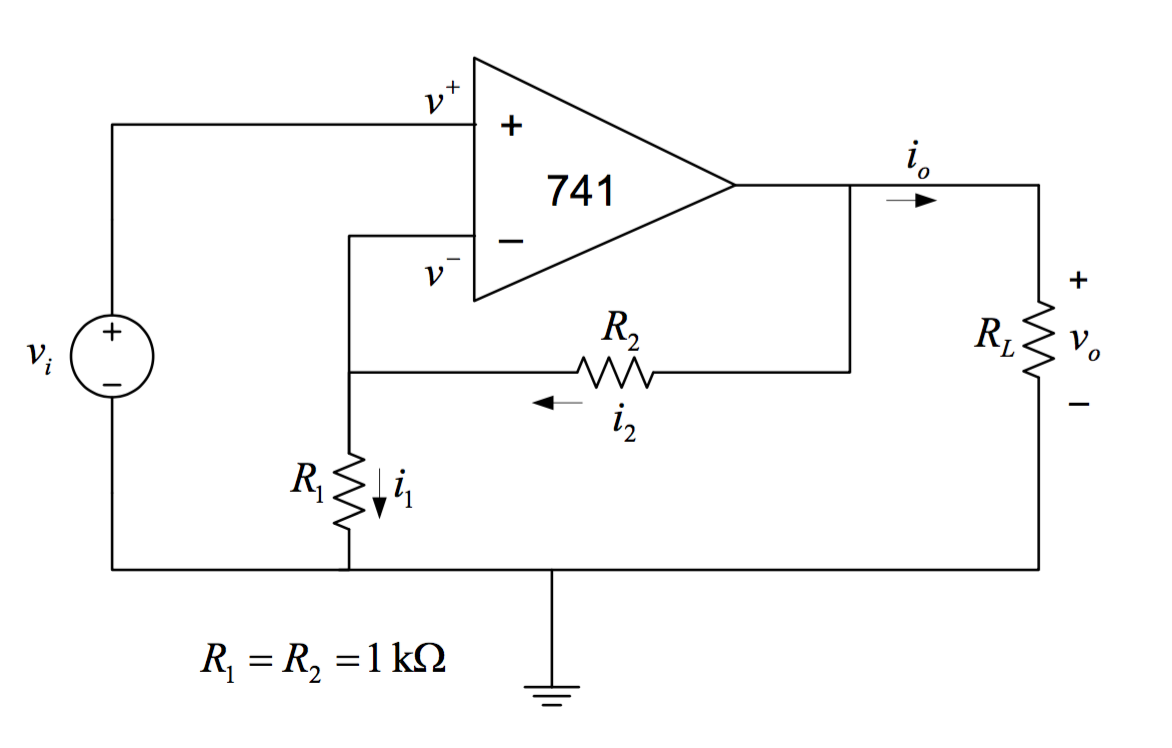
\includegraphics[width=0.475\linewidth]{graphics/vcvs-schematic}
		\label{fig:vcvs}
	}
	\subfigure[VCCS with $K = 1$ when $R_L = \SI{1}{\kilo\ohm}$]
	{
		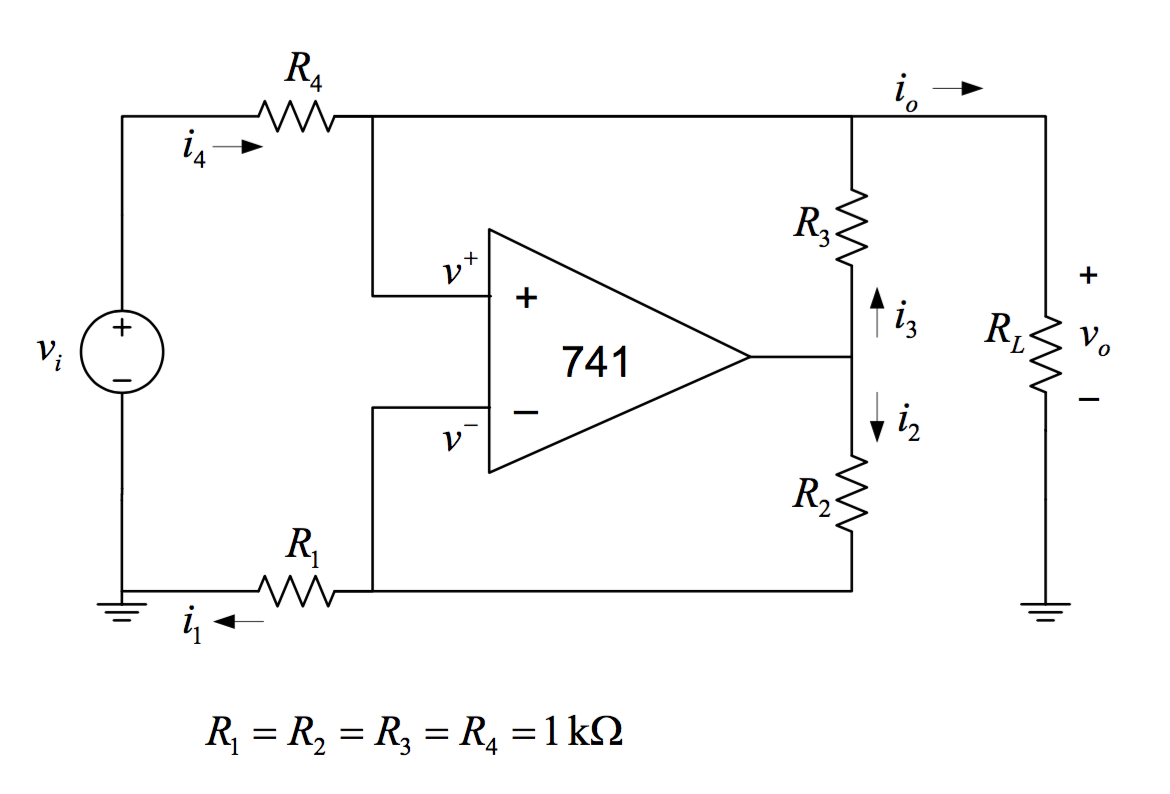
\includegraphics[width=0.475\linewidth]{graphics/vccs-schematic}
		\label{fig:vccs}
	}
	\caption{Circuits constructed in this lab \cite[p. 17]{lab-manual}}
	\label{fig:schematics}
\end{figure}

Since the VCVS is constructed as a non-inverting amplifier its governing equation is:
\begin{equation}\label{eq:vcvs}
	V_0 = V_i \left( {R_2 \over R_1} + 1 \right) = K V_i.
\end{equation}

Careful application of Kirchoff's Laws yields the following relation for the VCCS:
\begin{equation*}\label{eq:vccs}
	I_o = {V_i \over R}
\end{equation*}
where $R_1 = R_2 = R_3 = R_4 = R$.
The output voltage is constrained to:
\begin{equation}\label{eq:max-vccs}
	{V_{cc}^- \over 2} < V_i < {V_{cc}^+ \over 2}
\end{equation}
when $R_L = R$.